\documentclass[tikz,border=0pt]{standalone}
\usepackage{tikz}
\usetikzlibrary{arrows.meta,positioning,fit,calc}
\begin{document}
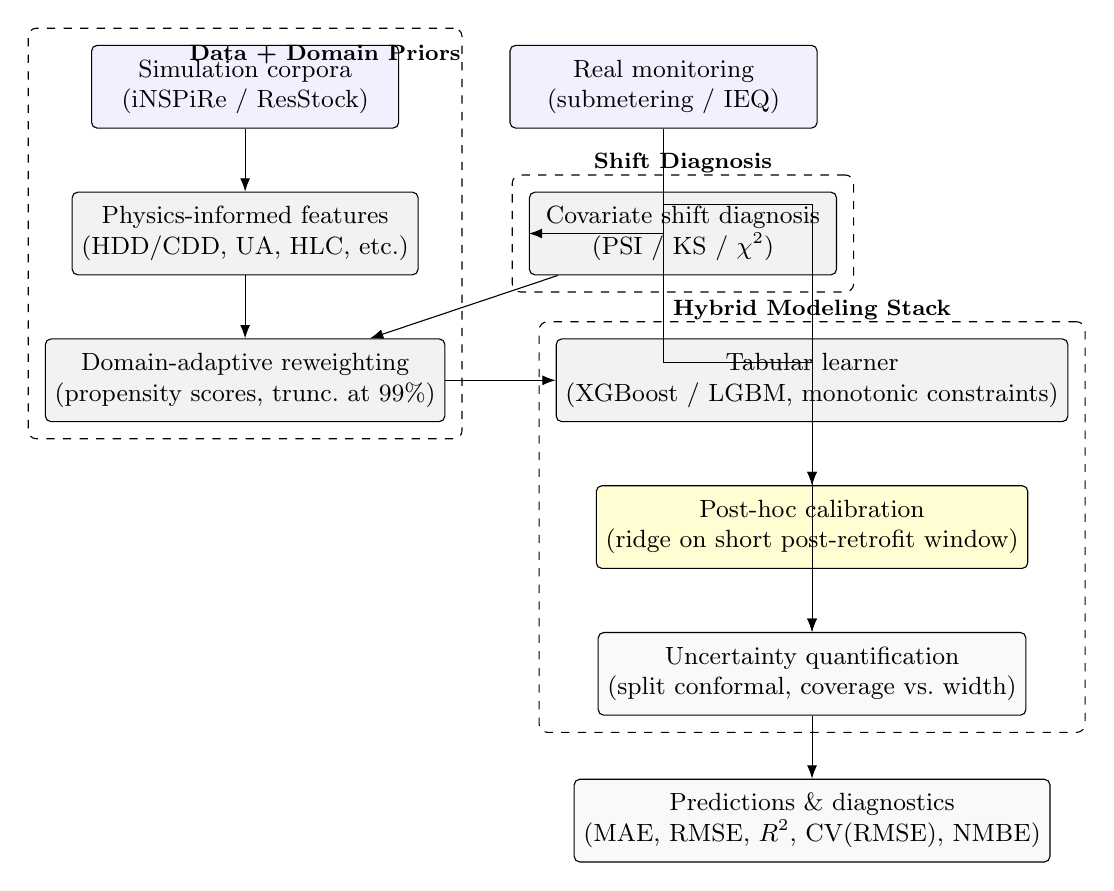
\begin{tikzpicture}[node distance=8mm and 14mm, >=LaTeX, font=\small]
  \tikzstyle{block}=[draw, rounded corners=2pt, align=center, minimum width=3.9cm, minimum height=1.05cm, fill=gray!5]
  \tikzstyle{data}=[block, fill=blue!6]
  \tikzstyle{proc}=[block, fill=gray!10]
  \tikzstyle{hl}=[block, fill=yellow!18]
  \tikzstyle{groupbox}=[draw, dashed, inner sep=6pt, rounded corners=3pt]

  % ------- nodes -------
  \node[data]    (sim)  {Simulation corpora\\(iNSPiRe / ResStock)};
  \node[data, right=of sim] (real) {Real monitoring\\(submetering / IEQ)};
  
  \node[proc, below=of sim] (fea)  {Physics-informed features\\(HDD/CDD, UA, HLC, etc.)};
  \node[proc, right=of fea] (shift) {Covariate shift diagnosis\\(PSI / KS / $\chi^2$)};
  
  \node[proc, below=of fea] (rew)  {Domain-adaptive reweighting\\(propensity scores, trunc.\ at 99\%)};
  \node[proc, right=of rew] (gbm)  {Tabular learner\\(XGBoost / LGBM, monotonic constraints)};
  
  \node[hl, below=of gbm]   (cal)  {Post-hoc calibration\\(ridge on short post-retrofit window)};
  \node[block, below=of cal] (uq)  {Uncertainty quantification\\(split conformal, coverage vs.\ width)};
  \node[block, below=of uq]  (pred) {Predictions \& diagnostics\\(MAE, RMSE, $R^2$, CV(RMSE), NMBE)};

  % group boxes
  \node[groupbox, fit=(sim)(fea)(rew)] (g1) {};
  \node[groupbox, fit=(shift)] (g2) {};
  \node[groupbox, fit=(gbm)(cal)(uq)] (g3) {};

  % group labels
  \node[above left=-1mm and -1mm of g1.north east, anchor=north east] {\footnotesize \textbf{Data + Domain Priors}};
  \node[above=-1mm of g2.north] {\footnotesize \textbf{Shift Diagnosis}};
  \node[above=-1mm of g3.north] {\footnotesize \textbf{Hybrid Modeling Stack}};

  % ------- arrows -------
  \draw[->] (sim) -- (fea);
  \draw[->] (real) |- (shift);
  \draw[->] (fea) -- (rew);
  \draw[->] (shift) -- (rew);
  \draw[->] (rew) -- (gbm);
  \draw[->] (gbm) -- (cal);
  \draw[->] (cal) -- (uq);
  \draw[->] (uq) -- (pred);

  % references to real data for calibration & UQ
  \draw[->] (real) |- +(0,-1.5) -| (cal);
  \draw[->] (real) |- +(0,-3.5) -| (uq);
\end{tikzpicture}
\end{document}
